\chapter{Specifikacija programske potpore}
		
	\section{Funkcionalni zahtjevi}

			%\textbf{\textit{dio 1. revizije}}\\
					
			\noindent \textbf{Dionici:}
			
			\begin{packed_enum}
				
				\item Vlasnik (naručitelj)
				\item Administrator
				\item Korisnici			
				\item Donatori
				\item Razvojni tim
				
			\end{packed_enum}
			
			\noindent \textbf{Aktori i njihovi funkcionalni zahtjevi:}
			
			
			\begin{packed_enum}
			
				\item  \underbar{Korisnik (inicijator) može:}
				
				\begin{packed_enum}
					\item stvoriti novi korisnički račun za koji su mu potrebni ime, prezime, lokacija, mail adresa i lozinka
					\item prijaviti se u sustav koristeći mail adresu i lozinku
					\item odjaviti se iz sustava
					\item pregledavati sve aktivne oglase
					\item pregledavati preporučene oglase
					\item pregledavati detalje oglasa
					\item filtrirati sve aktivne ili preporučene oglase po kategorijama i potkategorijama
					\item pregledavati osobne podatke
					\item uređivati osobne podatke
					\item izbrisati račun
					\item pregledavati podatke o svojoj djeci i njihovim praćenim kategorijama
					\item uređivati podatke o svojoj djeci i njihovim praćenim kategorijama
					\item dodavati podatke o svojoj djeci i njihovim praćenim kategorijama
					\item brisati podatke o svojoj djeci	
					
				\end{packed_enum}

				\eject

				\item  \underbar{Donator (inicijator) može:}
				
				\begin{packed_enum}
					\item stvoriti novi korisnički račun za koji su mu potrebni ime, prezime, lokacija, mail adresa i lozinka
					\item prijaviti se u sustav koristeći mail adresu i lozinku
					\item odjaviti se iz sustava
					\item pregledavati sve aktivne oglase
					\item pregledavati preporučene oglase
					\item pregledavati detalje oglasa
					\item filtrirati sve aktivne ili preporučene oglase po kategorijama i potkategorijama
					\item pregledavati osobne podatke
					\item uređivati osobne podatke
					\item izbrisati račun
					\item pregledavati podatke o svojoj djeci i njihovim praćenim kategorijama
					\item uređivati podatke o svojoj djeci i njihovim praćenim kategorijama
					\item dodavati podatke o svojoj djeci i njihovim praćenim kategorijama
					\item brisati podatke o svojoj djeci
					\item prihvatiti ili odbiti ponovno doniranje primljene donacije
					\item kreirati oglase za donacije
					\item uređivati svoje oglase za donacije 
					\item zatvarati svoje oglase za donacije
					\item pregledavati svoje oglase
				\end{packed_enum}

				\item  \underbar{Administrator (inicijator) može:}
				
				\begin{packed_enum}
					\item prijaviti se u sustav koristeći mail adresu i lozinku
					\item odjaviti se iz sustava
					\item pregledavati sve aktivne oglase
					\item pregledavati detalje oglasa
					\item pregledavati korisnike
					\item dodijeliti korisnicima ovlast za kreiranje oglasa
					\item oduzeti korisnicima ovlast za kreiranje oglasa
					\item pregledavati neobjavljene oglase
					\item prihvatiti i objaviti novostvorene oglase
					\item poslati novostvorene oglase na doradu
					\item odbiti novostvorene oglase
					\item kreirati nove kategorije i potkategorije
					
				\end{packed_enum}

				\eject

				\item  \underbar{Baza podataka (sudionik):}
				
				\begin{packed_enum}
					
					\item pohranjuje podatke o računima korisnika
					\item pohranjuje podatke o djeci korisnika
					\item pohranjuje sve podatke o donacijama
					
				\end{packed_enum}
			\end{packed_enum}
			
			\eject 
			
			
				
			\subsection{Obrasci uporabe}
				
				%\textbf{\textit{dio 1. revizije}}
				
				\subsubsection{Opis obrazaca uporabe}			

					\noindent \underbar{\textbf{UC1 - Registracija}}
					\begin{packed_item}
	
						\item \textbf{Glavni sudionik: }Korisnik
						\item  \textbf{Cilj:} Stvaranje računa
						\item  \textbf{Sudionici:} Baza podataka
						\item  \textbf{Preduvjet:} -
						\item  \textbf{Opis osnovnog tijeka:}
						
						\item[] \begin{packed_enum}
							\item Korisnik je na početnoj stranici odabrao opciju za registraciju
							\item Sustav prikazuje polja za unos
							\item Korisnik unosi potrebne podatke
							\item Sustav validira unesene podatke
							\item Korisnik potvrđuje unos podataka
							\item Sustav ažurira podatke u bazi i na mail adresu korisnika šalje potvrdu o uspješnoj registraciji
						\end{packed_enum}
						
						\item  \textbf{Opis mogućih odstupanja:}

						\item[] \begin{packed_item}
							\item[1.a] Korisnik ne odabire navedenu akciju - kraj scenarija
							\item[3.a] Korisnik odustaje od unosa u polja - kraj scenarija
							\item[4.a] Korisnik je unio podatake u neispravnom formatu
							\item[] \begin{packed_enum}
								\item Sustav upozorava korisika o neispravnom formatu podataka - scenarij nastavlja korakom 3 
							\end{packed_enum}	
							\item[6.a] Sustav utvrđuje da unešeni podaci nisu ispravni
							\item[] \begin{packed_enum}
								\item Sustav upozorava korisnika o pogrešnom unosu podataka - scenarij nastavlja korakom 3 
							\end{packed_enum}
							\item[6.b] Sustav utvrđuje da već postoji korisnik sa istom mail adresom
							\item[] \begin{packed_enum}
								\item Sustav upozorava korisnika o zauzetoj mail adresi - scenarij nastavlja korakom 3 
							\end{packed_enum}
							\item[6.c] Sustav ne uspije ažurirati podatke u bazi
							\item[] \begin{packed_enum}
								\item Sustav upozorava korisnika o neuspješnoj pohrani podataka - scenarij nastavlja korakom 3
							\end{packed_enum}					
						\end{packed_item}
					\end{packed_item}

					\eject

					\noindent \underbar{\textbf{UC2 - Prijava u sustav}}
					\begin{packed_item}
	
						\item \textbf{Glavni sudionik: }Korisnik ili administrator
						\item  \textbf{Cilj:} Pristup početnoj stranici
						\item  \textbf{Sudionici:} Baza podataka
						\item  \textbf{Preduvjet:} -

						\item  \textbf{Opis osnovnog tijeka:}
						
						\item[] \begin{packed_enum}
							\item Korisnik je na početnoj stranici odabrao opciju za prijavu
							\item Sustav prikazuje polja za unos
							\item Korisnik unosi potrebne podatke
							\item Sustav validira unesene podatke
							\item Korisnik potvrđuje unos podataka
							\item Sustav provjerava podatke u bazi i preusmjerava korisnika na početnu stranicu
						\end{packed_enum}

						\item  \textbf{Opis mogućih odstupanja:}

						\item[] \begin{packed_item}
							\item[1.a] Korisnik ne odabire navedenu akciju - kraj scenarija
							\item[3.a] Korisnik odustaje od unosa u polja - kraj scenarija
							\item[4.a] Korisnik je unio podatake u neispravnom formatu
							\item[] \begin{packed_enum}
								\item Sustav upozorava korisnika o neispravnom formatu podataka - scenarij nastavlja korakom 3
							\end{packed_enum}	
							\item[6.a] Sustav utvrđuje da unešeni podaci nisu ispravni
							\item[] \begin{packed_enum}
								\item Sustav upozorava korisnika o pogrešnom unosu podataka - scenarij nastavlja korakom 3 
							\end{packed_enum}
							\item[6.b] Sustav ne uspije ažurirati podatke u bazi
							\item[] \begin{packed_enum}
								\item Sustav upozorava korisnika o neuspješnoj provjeri podataka - scenarij nastavlja korakom 3
							\end{packed_enum}					
						\end{packed_item}
					\end{packed_item}

					\noindent \underbar{\textbf{UC3 - Odjava iz sustava}}
					\begin{packed_item}
	
						\item \textbf{Glavni sudionik: }Korisnik ili administrator
						\item  \textbf{Cilj:} Odjava korisnika
						\item  \textbf{Sudionici:} Baza podataka
						\item  \textbf{Preduvjet:} Korisnik je prijavljen u sustav
						\item  \textbf{Opis osnovnog tijeka:}
						
						\item[] \begin{packed_enum}
							\item Korisnik je odabrao opciju za odjavu
							\item Sustav pita korisnika želi li se sigurno odjaviti
							\item Korisnik potvrđuje da se želi odjaviti
							\item Sustav odjavljuje korisnika
						\end{packed_enum}

						\eject

						\item  \textbf{Opis mogućih odstupanja:}

						\item[] \begin{packed_item}
							\item[1.a] Korisnik ne odabire navedenu akciju - kraj scenarija
							\item[3.a] Korisnik odustaje od odjave - kraj scenarija
							\item[4.a] Sustav ne uspije odjaviti korisnika
							\item[] \begin{packed_enum}
								\item Sustav upozorava korisnika o neuspješnoj odjavi 
								\item
									\begin{packed_enum}
										\item Scenarij ponovno započinje
										\item Korisnik odustaje od odjave - kraj scenarija
									\end{packed_enum}
							\end{packed_enum}						
						\end{packed_item}
					\end{packed_item}

					\noindent \underbar{\textbf{UC4 - Pregled osobnih podataka}}
					\begin{packed_item}
	
						\item \textbf{Glavni sudionik: }Korisnik
						\item  \textbf{Cilj:} Pregled osobnih podataka unešenih u sustav
						\item  \textbf{Sudionici:} Baza podataka
						\item  \textbf{Preduvjet:} Korisnik je prijavljen u sustav
						\item  \textbf{Opis osnovnog tijeka:}
						
						\item[] \begin{packed_enum}
							\item Korisnik je odabrao opciju za prikaz osobnih podataka
							\item Sustav prikazuje korisnikove osobne podatke 
							\item Korisnik pregledava osobne podatke
						\end{packed_enum}
						\item  \textbf{Opis mogućih odstupanja:}

						\item[] \begin{packed_item}
							\item[1.a] Korisnik ne odabire navedenu akciju - kraj scenarija
							\item[2.a] Baza ne uspije poslati podatke o korisniku
							\item[] \begin{packed_enum}			
								\item Korisnik dobiva obavijest o neuspješnom dohvatu podataka
								\item
									\begin{packed_enum}
										\item Korisnik osvježava stranicu - scenarij nastavlja korakom 2
										\item Korisnik odustaje od pregleda osobnih podataka - kraj scenarija
									\end{packed_enum}						
							\end{packed_enum}	
						\end{packed_item}	
					\end{packed_item}

					\noindent \underbar{\textbf{UC5 - Uređivanje osobnih podataka}}
					\begin{packed_item}
	
						\item \textbf{Glavni sudionik: }Korisnik
						\item  \textbf{Cilj:} Promjena osobnih podataka unešenih u sustav
						\item  \textbf{Sudionici:} Baza podataka
						\item  \textbf{Preduvjet:} Korisnik je prijavljen u sustav
						\item  \textbf{Opis osnovnog tijeka:}
					
						\item[] \begin{packed_enum}
							\item Korisnik je odabrao opciju za uređivanje osobnih podataka
							\item Sustav prikazuje korisnikove osobne podatke 
							\item Korisnik mijenja osobne podatke
							\item Sustav validira unesene podatke
							\item Korisnik potvrđuje promjene
							\item Sustav ažurira podatke u bazi i preusmjerava korisnika na početnu stranicu
						\end{packed_enum}

						\eject

						\item  \textbf{Opis mogućih odstupanja:}

						\item[] \begin{packed_item}
							\item[1.a] Korisnik ne odabire navedenu akciju - kraj scenarija
							\item[3.a] Korisnik odustaje od unosa promjena - kraj scenarija
							\item[4.a] Korisnik je unio podatake u neispravnom formatu
							\item[] \begin{packed_enum}
								\item Sustav upozorava korisnika o neispravnom formatu podataka - scenarij nastavlja korakom 3 
							\end{packed_enum}	
							\item[6.a] Sustav utvrđuje da unešeni podaci nisu ispravni
							\item[] \begin{packed_enum}
								\item Sustav upozorava korisnika o pogrešnom unosu podataka - scenarij nastavlja korakom 3 
							\end{packed_enum}
							\item[6.b] Sustav ne uspije ažurirati podatke u bazi
							\item[] \begin{packed_enum}
								\item Sustav upozorava korisnika o neuspješnoj pohrani podataka - scenarij nastavlja korakom 3
							\end{packed_enum}					
						\end{packed_item}
					\end{packed_item}	
					
					\noindent \underbar{\textbf{UC6 - Brisanje korisničkog računa}}
					\begin{packed_item}
	
						\item \textbf{Glavni sudionik: }Korisnik
						\item  \textbf{Cilj:} Brisanje računa
						\item  \textbf{Sudionici:} Baza podataka
						\item  \textbf{Preduvjet:} Korisnik je prijavljen u sustav
						\item  \textbf{Opis osnovnog tijeka:}
						
						\item[] \begin{packed_enum}
							\item Korisnik je odabrao opciju za brisanje računa
							\item Sustav pita korisnika želi li sigurno obrisati svoj račun
							\item Korisnik potvrđuje da želi obrisati račun
							\item Sustav briše korisnikov račun
						\end{packed_enum}

						\item  \textbf{Opis mogućih odstupanja:}

						\item[] \begin{packed_item}
							\item[1.a] Korisnik ne odabire navedenu akciju - kraj scenarija
							\item[3.a] Korisnik odustaje od brisanja računa - kraj scenarija
							\item[4.a] Sustav ne uspije pobrisati korisnikov račun
							\item[] \begin{packed_enum}
								\item Sustav upozorava korisnika o neuspješnom brisanju
								\item
									\begin{packed_enum}
										\item Scenarij ponovno započinje
										\item Korisnik odustaje od brisanja računa - kraj scenarija
									\end{packed_enum}	
							\end{packed_enum}					
						\end{packed_item}
					\end{packed_item}	

					\noindent \underbar{\textbf{UC7 - Pregled podataka o djeci}}
					\begin{packed_item}
	
						\item \textbf{Glavni sudionik: }Korisnik
						\item  \textbf{Cilj:} Pregled podataka o djetetu korisnika
						\item  \textbf{Sudionici:} Baza podataka
						\item  \textbf{Preduvjet:} Korisnik je prijavljen u sustav i u sustavu postoje podaci o barem jednom korisnikovom djetetu
						\eject
						\item  \textbf{Opis osnovnog tijeka:}
						
						\item[] \begin{packed_enum}
							\item Korisnik je odabrao opciju za prikaz podataka o jednom od svoje djece
							\item Sustav prikazuje podatke o odabranom korisnikovom djetetu
							\item Korisnik pregledava podatke o djetetu
						\end{packed_enum}
						\item  \textbf{Opis mogućih odstupanja:}

						\item[] \begin{packed_item}
							\item[1.a] Korisnik ne odabire navedenu akciju - kraj scenarija
							\item[2.a] Baza ne uspije poslati podatke o djetetu
							\item[] \begin{packed_enum}	
								\item Korisnik dobiva obavijest o neuspješnom dohvatu podataka
								\item
									\begin{packed_enum}
										\item Korisnik osvježava stranicu - scenarij nastavlja korakom 2
										\item Korisnik odustaje od pregleda podataka o odabranom djetetu - kraj scenarija
									\end{packed_enum}	
							\end{packed_enum}	
						\end{packed_item}	
					\end{packed_item}

					\noindent \underbar{\textbf{UC8 - Uređivanje podataka o djeci}}
					\begin{packed_item}
	
						\item \textbf{Glavni sudionik: }Korisnik
						\item  \textbf{Cilj:} Promjena podataka o djetetu korisnika
						\item  \textbf{Sudionici:} Baza podataka
						\item  \textbf{Preduvjet:} Korisnik je prijavljen u sustav i u sustavu postoje podaci o barem jednom korisnikovom djetetu
						\item  \textbf{Opis osnovnog tijeka:}
						
						\item[] \begin{packed_enum}
							\item Korisnik je odabrao opciju za uređivanje podataka o jednom od svoje djece
							\item Sustav prikazuje podatke o odabranom korisnikovom djetetu
							\item Korisnik mijenja podatke o djetetu
							\item Sustav validira unesene podatke
							\item Korisnik potvrđuje promjene
							\item Sustav ažurira podatke u bazi i preusmjerava korisnika na početnu stranicu
						\end{packed_enum}

						\eject

						\item  \textbf{Opis mogućih odstupanja:}

						\item[] \begin{packed_item}
							\item[1.a] Korisnik ne odabire navedenu akciju - kraj scenarija
							\item[3.a] Korisnik odustaje od unosa promjena - kraj scenarija
							\item[4.a] Korisnik je unio podatake u neispravnom formatu
							\item[] \begin{packed_enum}
								\item Sustav upozorava korisnika o neispravnom formatu podataka - scenarij nastavlja korakom 3 
							\end{packed_enum}	
							\item[6.a] Sustav utvrđuje da unešeni podaci nisu ispravni
							\item[] \begin{packed_enum}
								\item Sustav upozorava korisnika o pogrešnom unosu podataka - scenarij nastavlja korakom 3 
							\end{packed_enum}
							\item[6.b] Sustav ne uspije ažurirati podatke u bazi
							\item[] \begin{packed_enum}
								\item Sustav upozorava korisnika o neuspješnoj pohrani podataka - scenarij nastavlja korakom 3
							\end{packed_enum}					
						\end{packed_item}
					\end{packed_item}

					\noindent \underbar{\textbf{UC9 - Dodavanje podataka o djeci}}
					\begin{packed_item}
	
						\item \textbf{Glavni sudionik: }Korisnik
						\item  \textbf{Cilj:} Dodavanje podataka o djetetu korisnika
						\item  \textbf{Sudionici:} Baza podataka
						\item  \textbf{Preduvjet:} Korisnik je prijavljen u sustav
						\item  \textbf{Opis osnovnog tijeka:}
						
						\item[] \begin{packed_enum}
							\item Korisnik je odabrao opciju za dodavanje podataka o jednom od svoje djece
							\item Sustav prikazuje polja za unos
							\item Korisnik unosi potrebne podatke
							\item Sustav validira unesene podatke
							\item Korisnik potvrđuje unos podataka
							\item Sustav ažurira podatke u bazi i preusmjerava korisnika na početnu stranicu
						\end{packed_enum}

						\eject

						\item  \textbf{Opis mogućih odstupanja:}

						\item[] \begin{packed_item}
							\item[1.a] Korisnik ne odabire navedenu akciju - kraj scenarija
							\item[3.a] Korisnik odustaje od unosa u polja - kraj scenarija
							\item[4.a] Korisnik je unio podatake u neispravnom formatu
							\item[] \begin{packed_enum}
								\item Sustav upozorava korisnika o neispravnom formatu podataka - scenarij nastavlja korakom 3 
							\end{packed_enum}	
							\item[6.a] Sustav utvrđuje da unešeni podaci nisu ispravni
							\item[] \begin{packed_enum}
								\item Sustav upozorava korisnika o pogrešnom unosu podataka - scenarij nastavlja korakom 3 
							\end{packed_enum}
							\item[6.b] Sustav ne uspije ažurirati podatke u bazi
							\item[] \begin{packed_enum}
								\item Sustav upozorava korisnika o neuspješnoj pohrani podataka - scenarij nastavlja korakom 3
							\end{packed_enum}					
						\end{packed_item}
					\end{packed_item}	

					\noindent \underbar{\textbf{UC10 - Brisanje podataka o djeci}}
					\begin{packed_item}
	
						\item \textbf{Glavni sudionik: }Korisnik
						\item  \textbf{Cilj:} Brisanje podataka o djetetu korisnika
						\item  \textbf{Sudionici:} Baza podataka
						\item  \textbf{Preduvjet:} Korisnik je prijavljen u sustav i u sustavu postoje podaci o barem jednom korisnikovom djetetu

						\item  \textbf{Opis osnovnog tijeka:}
						
						\item[] \begin{packed_enum}
							\item Korisnik je odabrao opciju za brisanje podataka o jednom od svoje djece
							\item Sustav pita korisnika želi li sigurno obrisati podatke o odabranome djetetu
							\item Korisnik potvrđuje da želi obrisati podatke o odabranome djetetu
							\item Sustav briše podatke o odabranome djetetu
						\end{packed_enum}

						\item  \textbf{Opis mogućih odstupanja:}

						\item[] \begin{packed_item}
							\item[1.a] Korisnik ne odabire navedenu akciju - kraj scenarija
							\item[3.a] Korisnik odustaje od brisanja podataka o odabranome djetetu - kraj scenarija
							\item[4.a] Sustav ne uspije obrisati podatke o odabranome djetetu
							\item[] \begin{packed_enum}
								\item Sustav upozorava korisnika o neuspješnom brisanju
								\item
									\begin{packed_enum}
										\item Scenarij ponovno započinje
										\item Korisnik odustaje od brisanja podataka - kraj scenarija
									\end{packed_enum}	
							\end{packed_enum}					
						\end{packed_item}
					\end{packed_item}	

					\eject

					\noindent \underbar{\textbf{UC11 - Pregled aktivnih oglasa}}
					\begin{packed_item}
	
						\item \textbf{Glavni sudionik: }Korisnik ili administrator
						\item  \textbf{Cilj:} Pregled svih aktivnih oglasa
						\item  \textbf{Sudionici:} Baza podataka
						\item  \textbf{Preduvjet:} Korisnik je prijavljen u sustav
						\item  \textbf{Opis osnovnog tijeka:}
						
						\item[] \begin{packed_enum}
							\item Korisnik je otišao na početnu stranicu
							\item Sustav prikazuje aktivne oglase
							\item Korisnik pregledava oglase
						\end{packed_enum}
						\item  \textbf{Opis mogućih odstupanja:}

						\item[] \begin{packed_item}
							\item[1.a] Korisnik ne odlazi na početnu stranicu - kraj scenarija
							\item[2.a] Baza ne uspije poslati podatke o aktivnim oglasima
							\item[] \begin{packed_enum}
								
								\item Korisnik dobiva obavijest o neuspješnom dohvatu podataka
								\item
									\begin{packed_enum}
										\item Korisnik osvježava stranicu - scenarij nastavlja korakom 2
										\item Korisnik odustaje od pregleda aktivnih oglasa - kraj scenarija
									\end{packed_enum}
							
							\end{packed_enum}	
							\item[2.b] Ne postoji nijedan aktivan oglas
							\item[] \begin{packed_enum}
								
								\item Korisnik dobiva obavijest o nepostojanju aktivnih oglasa
								\item Korisnik odustaje od pregleda aktivnih oglasa - kraj scenarija
							
							\end{packed_enum}
						\end{packed_item}	
					\end{packed_item}

					\noindent \underbar{\textbf{UC12 - Pregled preporučenih oglasa}}
					\begin{packed_item}
	
						\item \textbf{Glavni sudionik: }Korisnik
						\item  \textbf{Cilj:} Pregled oglasa personaliziranih korisniku
						\item  \textbf{Sudionici:} Baza podataka
						\item  \textbf{Preduvjet:} Korisnik je prijavljen u sustav
						
						
						\item  \textbf{Opis osnovnog tijeka:}
						
						\item[] \begin{packed_enum}
							\item Korisnik je odabrao opciju za prikaz preporučenih oglasa
							\item Sustav prikazuje preporučene oglase
							\item Korisnik pregledava oglase
						\end{packed_enum}

						\eject

						\item  \textbf{Opis mogućih odstupanja:}

						\item[] \begin{packed_item}
							\item[1.a] Korisnik ne odabire navedenu akciju - kraj scenarija
							\item[2.a] Baza ne uspije poslati podatke o preporučenim oglasima
							\item[] \begin{packed_enum}		
								\item Korisnik dobiva obavijest o neuspješnom dohvatu podataka
								\item
									\begin{packed_enum}
										\item Korisnik osvježava stranicu - scenarij nastavlja korakom 2
										\item Korisnik odustaje od pregleda preporučenih oglasa - kraj scenarija
									\end{packed_enum}							
							\end{packed_enum}	
							\item[2.b] Ne postoje oglasi koji odgovaraju korisnikovim željama
							\item[] \begin{packed_enum}		
								\item Korisnik dobiva obavijest o manjku odgovarajućih oglasa
								\item Korisnik odustaje od pregleda preporučenih oglasa - kraj scenarija							
							\end{packed_enum}	
						\end{packed_item}	
					\end{packed_item}

					\noindent \underbar{\textbf{UC13 - Filtriranje oglasa}}
					\begin{packed_item}
	
						\item \textbf{Glavni sudionik: }Korisnik
						\item  \textbf{Cilj:} Pregled oglasa iz određene kategorije/potkategorije
						\item  \textbf{Sudionici:} Baza podataka
						\item  \textbf{Preduvjet:} Korisnik je prijavljen u sustav
						\item  \textbf{Opis osnovnog tijeka:}
						
						\item[] \begin{packed_enum}
							\item Korisnik je odabrao opciju za filtriranje aktivnih ili preporučenih oglasa po određenom parametru
							\item Sustav prikazuje oglase koji odgovaraju odabranim kategorijama i/ili potkategorijama
							\item Korisnik pregledava oglase
						\end{packed_enum}
						
						\item  \textbf{Opis mogućih odstupanja:}

						\item[] \begin{packed_item}
							\item[1.a] Korisnik ne odabire navedenu akciju - kraj scenarija
							\item[2.a] Baza ne uspije poslati podatke o odgovarajućim oglasima
							\item[] \begin{packed_enum}							
								\item Korisnik dobiva obavijest o neuspješnom dohvatu podataka
								\item
									\begin{packed_enum}
										\item Scenarij ponovno započinje
										\item Korisnik odustaje od filtriranja - kraj scenarija
									\end{packed_enum}			
							\end{packed_enum}	

							\item[2.b] Ne postoje oglasi koji odgovaraju zadanim opcijama filtriranja
							\item[] \begin{packed_enum}							
								\item Korisnik dobiva obavijest o manjku odgovarajućih oglasa
								\item
									\begin{packed_enum}
										\item Korisnik mijenja opcije filtriranja - scenarij nastavlja korakom 2
										\item Korisnik odustaje od filtriranja - kraj scenarija
									\end{packed_enum}							
							\end{packed_enum}	
						\end{packed_item}
					\end{packed_item}

					\eject

					\noindent \underbar{\textbf{UC14 - Pregled detalja o oglasu}}
					\begin{packed_item}
	
						\item \textbf{Glavni sudionik: }Korisnik ili administrator
						\item  \textbf{Cilj:} Pregled detalja određene donacije
						\item  \textbf{Sudionici:} Baza podataka
						\item  \textbf{Preduvjet:} Korisnik je prijavljen u sustav i u sustavu postoje podaci o barem jednom oglasu
						\item  \textbf{Opis osnovnog tijeka:}
						
						\item[] \begin{packed_enum}
							\item Korisnik je odabrao opciju za prikaz detalja o određenoj donaciji
							\item Sustav prikazuje detalje o izabranoj donaciji
							\item Korisnik pregledava detaljne informacije o donaciji
						\end{packed_enum}

						\item  \textbf{Opis mogućih odstupanja:}

						\item[] \begin{packed_item}
							\item[1.a] Korisnik ne odabire navedenu akciju - kraj scenarija
							\item[2.a] Baza ne uspije poslati podatke o izabranoj donaciji
							\item[] \begin{packed_enum}
								
								\item Korisnik dobiva obavijest o neuspješnom dohvatu podataka
								\item
									\begin{packed_enum}
										\item Korisnik osvježava stranicu - scenarij nastavlja korakom 2
										\item Korisnik odustaje od pregleda detalja o oglasu - kraj scenarija
									\end{packed_enum}	
							
							\end{packed_enum}	
						\end{packed_item}	
					\end{packed_item}

					\noindent \underbar{\textbf{UC15 - Poticanje donacija}}
					\begin{packed_item}
	
						\item \textbf{Glavni sudionik: }Donator
						\item  \textbf{Cilj:} Podsjećanje donatora o mogućnosti doniranja primljenog predmeta
						\item  \textbf{Sudionici:} Baza podataka
						\item  \textbf{Preduvjet:} Donator je prijavljen u sustav i ima primljene donacije kojima je isteklo standardno vrijeme korištenja

						\item  \textbf{Opis osnovnog tijeka:}
						
						\item[] \begin{packed_enum}
							\item Sustav donatoru šalje obavijest o mogućnosti doniranja primljenog predmeta
							\item Donator prihvaća mogućnost doniranja predmeta i biva preusmjeren na kreiranje oglasa
						\end{packed_enum}

						\item  \textbf{Opis mogućih odstupanja:}

						\item[] \begin{packed_item}
							\item[2.a] Donator odbija mogućnost doniranja predmeta
							\item[] \begin{packed_enum}
								
								\item Obavijest o mogućnosti doniranja se više ne prikazuje - kraj scenarija
							
							\end{packed_enum}	
						\end{packed_item}
					\end{packed_item}

					\eject

					\noindent \underbar{\textbf{UC16 - Kreiranje oglasa}}
					\begin{packed_item}
	
						\item \textbf{Glavni sudionik: }Donator
						\item  \textbf{Cilj:} Stvaranje nove donacije
						\item  \textbf{Sudionici:} Baza podataka
						\item  \textbf{Preduvjet:} Donator je prijavljen u sustav
						\item  \textbf{Opis osnovnog tijeka:}
						
						\item[] \begin{packed_enum}
							\item Donator je odabrao opciju za stvaranje nove donacije
							\item Sustav prikazuje polja za unos
							\item Donator unosi potrebne podatke
							\item Sustav validira unesene podatke
							\item Donator potvrđuje unos podataka
							\item Sustav ažurira podatke u bazi i preusmjerava donatora na početnu stranicu
						\end{packed_enum}

						\item  \textbf{Opis mogućih odstupanja:}

						\item[] \begin{packed_item}
							\item[1.a] Donator ne odabire navedenu akciju - kraj scenarija
							\item[3.a] Donator odustaje od unosa u polja - kraj scenarija
							\item[4.a] Donator je unio podatake u neispravnom formatu
							\item[] \begin{packed_enum}
								\item Sustav upozorava donatora o neispravnom formatu podataka - scenarij nastavlja korakom 3
							\end{packed_enum}	
							\item[6.a] Sustav utvrđuje da unešeni podaci nisu ispravni
							\item[] \begin{packed_enum}
								\item Sustav upozorava donatora o pogrešnom unosu podataka - scenarij nastavlja korakom 3
							\end{packed_enum}	
							\item[6.b] Sustav ne uspije ažurirati podatke u bazi
							\item[] \begin{packed_enum}
								\item Sustav upozorava donatora o neuspješnoj pohrani podataka - scenarij nastavlja korakom 3
							\end{packed_enum}				
						\end{packed_item}
					\end{packed_item}				

					\noindent \underbar{\textbf{UC17 - Uređivanje oglasa}}
					\begin{packed_item}
	
						\item \textbf{Glavni sudionik: }Donator
						\item  \textbf{Cilj:} Izmjena podataka o donaciji
						\item  \textbf{Sudionici:} Baza podataka
						\item  \textbf{Preduvjet:} Donator je prijavljen u sustav i u sustavu postoje podaci o barem jednom oglasu koji korisnik treba doraditi
						
						\eject
						
						\item  \textbf{Opis osnovnog tijeka:}
						
						\item[] \begin{packed_enum}
							\item Donator odabire oglas koji želi uređivati
							\item Sustav prikazuje oglas
							\item Donator odabere opciju za uređivanje oglasa
							\item Sustav prikazuje podatke o donaciji
							\item Donator mijenja podatke o donaciji
							\item Sustav validira unesene podatke
							\item Donator potvrđuje promjene
							\item Sustav ažurira podatke u bazi i preusmjerava donatora na početnu stranicu
						\end{packed_enum}

						\item  \textbf{Opis mogućih odstupanja:}

						\item[] \begin{packed_item}
							\item[1.a] Donator ne odabire navedenu akciju - kraj scenarija
							\item[2.a] Baza ne uspije poslati podatke o izabranom oglasu
							\item[] \begin{packed_enum}
								
								\item Donator dobiva obavijest o neuspješnom dohvatu podataka
								\item
									\begin{packed_enum}
										\item Donator osvježava stranicu - scenarij nastavlja korakom 2
										\item Donator odustaje od uređivanja oglasa - kraj scenarija
									\end{packed_enum}
							\end{packed_enum}
							\item[5.a] Donator odustaje od unosa promjena - kraj scenarija
							\item[6.a] Donator je unio podatake u neispravnom formatu
							\item[] \begin{packed_enum}
								\item Sustav upozorava donatora o neispravnom formatu podataka - scenarij nastavlja korakom 5
							\end{packed_enum}	
							\item[8.a] Sustav utvrđuje da unešeni podaci nisu ispravni
							\item[] \begin{packed_enum}
								\item Sustav upozorava donatora o pogrešnom unosu podataka - scenarij nastavlja korakom 5
							\end{packed_enum}
							\item[8.b] Sustav ne uspije ažurirati podatke u bazi
							\item[] \begin{packed_enum}
								\item Sustav upozorava donatora o neuspješnoj pohrani podataka - scenarij nastavlja korakom 5 
							\end{packed_enum}					
						\end{packed_item}
					\end{packed_item}

					\noindent \underbar{\textbf{UC18 - Zatvaranje oglasa}}
					\begin{packed_item}
	
						\item \textbf{Glavni sudionik: }Donator
						\item  \textbf{Cilj:} Zatvaranje trenutno aktivnog oglasa
						\item  \textbf{Sudionici:} Baza podataka
						\item  \textbf{Preduvjet:} Donator je prijavljen u sustav i u sustavu postoje podaci o barem jednom aktivnom oglasu korisnika
						
						\eject

						\item  \textbf{Opis osnovnog tijeka:}
						
						\item[] \begin{packed_enum}
							\item Donator odabire oglas koji želi zatvoriti
							\item Sustav prikazuje oglas
							\item Donator odabere opciju za zatvaranje oglasa
							\item Sustav pita donatora želi li sigurno zatvoriti odabrani oglas
							\item Donator potvrđuje da želi zatvoriti oglas
							\item Sustav ažurira podatke u bazi i preusmjerava donatora na početnu stranicu
						\end{packed_enum}

						\item  \textbf{Opis mogućih odstupanja:}

						\item[] \begin{packed_item}
							\item[1.a] Donator ne odabire navedenu akciju - kraj scenarija
							\item[2.a] Baza ne uspije poslati podatke o izabranom oglasu
							\item[] \begin{packed_enum}
								
								\item Donator dobiva obavijest o neuspješnom dohvatu podataka
								\item
									\begin{packed_enum}
										\item Donator osvježava stranicu - scenarij nastavlja korakom 2
										\item Donator odustaje od zatvaranja oglasa - kraj scenarija
									\end{packed_enum}
							\end{packed_enum}
							\item[3.a] Donator odustaje od zatvaranja odabranog oglasa
							\item[4.a] Sustav ne uspije ažurirati podatke u bazi
							\item[] \begin{packed_enum}
								\item Sustav upozorava donatora o neuspješnoj pohrani podataka
								\item
									\begin{packed_enum}
										\item Scenarij ponovno započinje
										\item Donator odustaje od zatvaranja oglasa - kraj scenarija
									\end{packed_enum}	
							\end{packed_enum}					
						\end{packed_item}
					\end{packed_item}	

					\noindent \underbar{\textbf{UC19 - Dodjela dozvole}}
					\begin{packed_item}
	
						\item \textbf{Glavni sudionik: }Administrator
						\item  \textbf{Cilj:} Dodjela dozvole za doniranje odabranome korisniku
						\item  \textbf{Sudionici:} Baza podataka
						\item  \textbf{Preduvjet:} Administrator je prijavljen u sustav i postoji barem jedan korisnik kojemu se može dodijeliti dozvola
						
						\item  \textbf{Opis osnovnog tijeka:}
						
						\item[] \begin{packed_enum}
							\item Administrator je odabrao opciju za dodjelu dozvole za doniranje odabranome korisniku
							\item Sustav pita administratora želi li sigurno dodijeliti dozvolu za doniranje odabranome korisniku
							\item Administrator potvrđuje da želi dodijeliti dozvolu
							\item Sustav ažurira podatke u bazi i preusmjerava administratora na početnu stranicu
						\end{packed_enum}

						\eject
						
						\item  \textbf{Opis mogućih odstupanja:}

						\item[] \begin{packed_item}
							\item[1.a] Administrator ne odabire navedenu akciju - kraj scenarija
							\item[3.a] Administrator odustaje od dodjele dozvole
							\item[4.a] Sustav ne uspije ažurirati podatke u bazi
							\item[] \begin{packed_enum}
								\item Sustav upozorava administratora o neuspješnoj pohrani podataka
								\item
									\begin{packed_enum}
										\item Scenarij ponovno započinje 
										\item Administrator odustaje od dodjele dozvole odabranome korisniku - kraj scenarija
									\end{packed_enum}
							\end{packed_enum}					
						\end{packed_item}
					\end{packed_item}

					\noindent \underbar{\textbf{UC20 - Uklanjanje dozvole}}
					\begin{packed_item}
	
						\item \textbf{Glavni sudionik: }Administrator
						\item  \textbf{Cilj:} Uklanjanje dozvole za doniranje odabranome korisniku
						\item  \textbf{Sudionici:} Baza podataka
						\item  \textbf{Preduvjet:} Administrator je prijavljen u sustav i postoji barem jedan korisnik kojemu se može ukloniti dozvola
						
						\item  \textbf{Opis osnovnog tijeka:}
						
						\item[] \begin{packed_enum}
							\item Administrator je odabrao opciju za uklanjanje dozvole za doniranje odabranome korisniku
							\item Sustav pita administratora želi li sigurno ukloniti dozvolu za doniranje odabranome korisniku
							\item Administrator potvrđuje da želi ukloniti dozvolu
							\item Sustav ažurira podatke u bazi i preusmjerava administratora na početnu stranicu
						\end{packed_enum}

						\item  \textbf{Opis mogućih odstupanja:}

						\item[] \begin{packed_item}
							\item[1.a] Administrator ne odabire navedenu akciju - kraj scenarija
							\item[3.a] Administrator odustaje od uklanjanja dozvole
							\item[4.a] Sustav ne uspije ažurirati podatke u bazi
							\item[] \begin{packed_enum}
								\item Sustav upozorava administratora o neuspješnoj pohrani podataka
								\item
									\begin{packed_enum}
										\item Scenarij ponovno započinje 
										\item Administrator odustaje od uklanjanja dozvole odabranome korisniku - kraj scenarija
									\end{packed_enum}
							\end{packed_enum}					
						\end{packed_item}
					\end{packed_item}

					\eject

					\noindent \underbar{\textbf{UC21 - Pregled neobjavljenih oglasa}}
					\begin{packed_item}
	
						\item \textbf{Glavni sudionik: }Administrator
						\item  \textbf{Cilj:} Pregled svih neobjavljenih oglasa
						\item  \textbf{Sudionici:} Baza podataka
						\item  \textbf{Preduvjet:} Administrator je prijavljen u sustav
						\item  \textbf{Opis osnovnog tijeka:}
						
						\item[] \begin{packed_enum}
							\item Administrator je odabrao opciju za prikaz neobjavljenih oglasa
							\item Sustav prikazuje neobjavljene oglase
							\item Administrator pregledava oglase
						\end{packed_enum}

						\item  \textbf{Opis mogućih odstupanja:}

						\item[] \begin{packed_item}
							\item[1.a] Administrator ne odabire navedenu akciju - kraj scenarija
							\item[2.a] Baza ne uspije poslati podatke o neobjavljenim oglasima
							\item[] \begin{packed_enum}
								
								\item Administrator dobiva obavijest o neuspješnom dohvatu podataka
								\item
									\begin{packed_enum}
										\item Administrator osvježava stranicu - scenarij nastavlja korakom 2
										\item Administrator odustaje od pregleda neobjavljenih oglasa - kraj scenarija
									\end{packed_enum}
							
							\end{packed_enum}	
							\item[2.b] Ne postoji nijedan neobjavljeni oglas
							\item[] \begin{packed_enum}
								
								\item Administrator dobiva obavijest o nepostojanju neobjavljenih oglasa
								\item Administrator odustaje od pregleda neobjavljenih oglasa - kraj scenarija
							
							\end{packed_enum}
						\end{packed_item}	
					\end{packed_item}
					
					\noindent \underbar{\textbf{UC22 - Odobravanje oglasa}}
					\begin{packed_item}
	
						\item \textbf{Glavni sudionik: }Administrator
						\item  \textbf{Cilj:} Odobravanje i objava donacije
						\item  \textbf{Sudionici:} Baza podataka
						\item  \textbf{Preduvjet:} Administrator je prijavljen u sustav i barem jedan oglas čeka odobrenje
						\item  \textbf{Opis osnovnog tijeka:}
						
						\item[] \begin{packed_enum}
							\item Administrator odabire oglas koji čeka odobrenje
							\item Sustav prikazuje oglas
							\item Administrator provjerava oglas i odabire opciju za odobravanje oglasa
							\item Sustav pita administratora želi li sigurno odobriti navedeni oglas
							\item Administrator potvrđuje da želi odobriti oglas
							\item Sustav ažurira podatke u bazi, objavljuje oglas i preusmjerava administratora na početnu stranicu
						\end{packed_enum}

						\item  \textbf{Opis mogućih odstupanja:}

						\item[] \begin{packed_item}
							\item[2.a] Baza ne uspije poslati podatke o izabranom oglasu
							\item[] \begin{packed_enum}
								
								\item Administrator dobiva obavijest o neuspješnom dohvatu podataka
								\item
									\begin{packed_enum}
										\item Administrator osvježava stranicu - scenarij nastavlja korakom 2
										\item Administrator odustaje od odobravanja oglasa - kraj scenarija
									\end{packed_enum}	
							\end{packed_enum}
							\item[5.a] Administrator odustaje od odobravanja navedenog oglasa
							\item[6.a] Sustav ne uspije ažurirati podatke u bazi
							\item[] \begin{packed_enum}
								\item Sustav upozorava administratora o neuspješnoj pohrani podataka 
								\item
									\begin{packed_enum}
										\item Scenarij ponovno započinje
										\item Administrator odustaje od odobravanja oglasa - kraj scenarija
									\end{packed_enum}
							\end{packed_enum}					
						\end{packed_item}
					\end{packed_item}

					\noindent \underbar{\textbf{UC23 - Slanje oglasa na doradu}}
					\begin{packed_item}
	
						\item \textbf{Glavni sudionik: }Administrator
						\item  \textbf{Cilj:} Slanje oglasa natrag donatoru na doradu
						\item  \textbf{Sudionici:} Baza podataka
						\item  \textbf{Preduvjet:} Administrator je prijavljen u sustav i barem jedan oglas čeka odobrenje
						\item  \textbf{Opis osnovnog tijeka:}
						
						\item[] \begin{packed_enum}
							\item Administrator odabire oglas koji čeka odobrenje
							\item Sustav prikazuje oglas
							\item Administrator provjerava oglas i odabire opciju za slanje oglasa na doradu
							\item Sustav pita administratora želi li sigurno poslati navedeni oglas na doradu
							\item Administrator potvrđuje da želi poslati oglas na doradu
							\item Sustav ažurira podatke u bazi i preusmjerava administratora na početnu stranicu
						\end{packed_enum}

						\eject

						\item  \textbf{Opis mogućih odstupanja:}

						\item[] \begin{packed_item}
							\item[2.a] Baza ne uspije poslati podatke o izabranom oglasu
							\item[] \begin{packed_enum}
								
								\item Administrator dobiva obavijest o neuspješnom dohvatu podataka
								\item
									\begin{packed_enum}
										\item Administrator osvježava stranicu - scenarij nastavlja korakom 2
										\item Administrator odustaje od slanja oglasa na doradu - kraj scenarija
									\end{packed_enum}	
							\end{packed_enum}
							\item[5.a]  Administrator odustaje od slanja navedenog oglasa na doradu
							\item[6.a] Sustav ne uspije ažurirati podatke u bazi
							\item[] \begin{packed_enum}
								\item Sustav upozorava administratora o neuspješnoj pohrani podataka 
								\item
									\begin{packed_enum}
										\item Scenarij ponovno započinje
										\item Administrator odustaje od slanja oglasa na doradu - kraj scenarija
									\end{packed_enum}
								\end{packed_enum}					
						\end{packed_item}
					\end{packed_item}

					\noindent \underbar{\textbf{UC24 - Odbijanje oglasa}}
					\begin{packed_item}
	
						\item \textbf{Glavni sudionik: }Administrator
						\item  \textbf{Cilj:} Odbijanje oglasa
						\item  \textbf{Sudionici:} Baza podataka
						\item  \textbf{Preduvjet:} Administrator je prijavljen u sustav i barem jedan oglas čeka odobrenje
						\item  \textbf{Opis osnovnog tijeka:}
						
						\item[] \begin{packed_enum}
							\item Administrator odabire oglas koji čeka odobrenje
							\item Sustav prikazuje oglas
							\item Administrator provjerava oglas i odabire opciju za odbijanje oglasa
							\item Sustav pita administratora želi li sigurno odbiti navedeni oglas
							\item Administrator potvrđuje da želi odbiti navedeni oglas
							\item Sustav ažurira podatke u bazi i preusmjerava administratora na početnu stranicu
						\end{packed_enum}

						\eject

						\item  \textbf{Opis mogućih odstupanja:}

						\item[] \begin{packed_item}
							\item[2.a] Baza ne uspije poslati podatke o izabranom oglasu
							\item[] \begin{packed_enum}
								
								\item Administrator dobiva obavijest o neuspješnom dohvatu podataka
								\item
									\begin{packed_enum}
										\item Administrator osvježava stranicu - scenarij nastavlja korakom 2
										\item Administrator odustaje od odbijanja oglasa - kraj scenarija
									\end{packed_enum}	
							\end{packed_enum}
							\item[5.a] Administrator odustaje od odbijanja navedenog oglasa
							\item[6.a] Sustav ne uspije ažurirati podatke u bazi
							\item[] \begin{packed_enum}
								\item Sustav upozorava administratora o neuspješnoj pohrani podataka 
								\item
									\begin{packed_enum}
										\item Scenarij ponovno započinje
										\item Administrator odustaje od odbijanja oglasa - kraj scenarija
									\end{packed_enum}
								\end{packed_enum}					
						\end{packed_item}
					\end{packed_item}

					\noindent \underbar{\textbf{UC25 - Dodavanje kategorija}}
					\begin{packed_item}
	
						\item \textbf{Glavni sudionik: }Administrator
						\item  \textbf{Cilj:} Dodavanje nove kategorije u sustav
						\item  \textbf{Sudionici:} Baza podataka
						\item  \textbf{Preduvjet:} Administrator je prijavljen u sustav
						\item  \textbf{Opis osnovnog tijeka:}
						
						\item[] \begin{packed_enum}
							\item Administrator je odabrao opciju za dodavanje kategorija
							\item Sustav prikazuje polja za unos
							\item Administrator unosi potrebne podatke
							\item Sustav validira unesene podatke
							\item Administrator potvrđuje unos podataka
							\item Sustav administratora preusmjeri na početnu stranicu
						\end{packed_enum}
						\item  \textbf{Opis mogućih odstupanja:}

						\item[] \begin{packed_item}
							\item[1.a] Administrator ne odabire navedenu akciju - kraj scenarija
							\item[3.a] Administrator odustaje od unosa u polja - kraj scenarija
							\item[4.a] Administrator je unio podatake u neispravnom formatu
							\item[] \begin{packed_enum}
								\item Sustav upozorava administratora o neispravnom formatu podataka - scenarij nastavlja korakom 3
							\end{packed_enum}	
							\item[6.a] Sustav utvrđuje da unešeni podaci nisu ispravni
							\item[] \begin{packed_enum}
								\item Sustav upozorava administratora o pogrešnom unosu podataka - scenarij nastavlja korakom 3
							\end{packed_enum}
							\item[6.b] Sustav ne uspije ažurirati podatke u bazi
							\item[] \begin{packed_enum}
								\item Sustav upozorava administratora o neuspješnoj pohrani podataka - scenarij nastavlja korakom 3
							\end{packed_enum}						
						\end{packed_item}
					\end{packed_item}

					\eject

					\noindent \underbar{\textbf{UC26 - Dodavanje potkategorija}}
					\begin{packed_item}
	
						\item \textbf{Glavni sudionik: }Administrator
						\item  \textbf{Cilj:} Dodavanje nove potkategorije u sustav
						\item  \textbf{Sudionici:} Baza podataka
						\item  \textbf{Preduvjet:} Administrator je prijavljen u sustav
						
						\item  \textbf{Opis osnovnog tijeka:}
						
						\item[] \begin{packed_enum}
							\item Administrator je odabrao opciju za dodavanje potkategorija
							\item Sustav prikazuje polja za unos
							\item Administrator unosi potrebne podatke
							\item Sustav validira unesene podatke
							\item Administrator potvrđuje unos podataka
							\item Sustav administratora preusmjeri na početnu stranicu
						\end{packed_enum}			
						
						\item  \textbf{Opis mogućih odstupanja:}

						\item[] \begin{packed_item}
							\item[1.a] Administrator ne odabire navedenu akciju - kraj scenarija
							\item[3.a] Administrator odustaje od unosa u polja - kraj scenarija
							\item[4.a] Administrator je unio podatake u neispravnom formatu
							\item[] \begin{packed_enum}
								\item Sustav upozorava administratora o neispravnom formatu podataka - scenarij nastavlja korakom 3
							\end{packed_enum}	
							\item[6.a] Sustav utvrđuje da unešeni podaci nisu ispravni
							\item[] \begin{packed_enum}
								\item Sustav upozorava administratora o pogrešnom unosu podataka - scenarij nastavlja korakom 3
							\end{packed_enum}	
							\item[6.b] Sustav ne uspije ažurirati podatke u bazi
							\item[] \begin{packed_enum}
								\item Sustav upozorava administratora o neuspješnoj pohrani podataka - scenarij nastavlja korakom 3
							\end{packed_enum}				
						\end{packed_item}
					\end{packed_item}

					\noindent \underbar{\textbf{UC27 - Pregled korisnika}}
					\begin{packed_item}
	
						\item \textbf{Glavni sudionik: }Administrator
						\item  \textbf{Cilj:} Pregled svih korisnika
						\item  \textbf{Sudionici:} Baza podataka
						\item  \textbf{Preduvjet:} Administrator je prijavljen u sustav
						\item  \textbf{Opis osnovnog tijeka:}
						
						\item[] \begin{packed_enum}
							\item Administrator je odabrao opciju za prikaz svih korisika
							\item Sustav prikazuje sve korisnike
							\item Administrator pregledava korisnike
						\end{packed_enum}
						
						\eject

						\item  \textbf{Opis mogućih odstupanja:}

						\item[] \begin{packed_item}
							\item[1.a] Administrator ne odabire navedenu akciju - kraj scenarija
							\item[2.a] Baza ne uspije poslati podatke o korisnicima
							\item[] \begin{packed_enum}
								
								\item Administrator dobiva obavijest o neuspješnom dohvatu podataka o korisnicima
								\item
									\begin{packed_enum}
										\item Administrator osvježava stranicu - scenarij nastavlja korakom 2
										\item Administrator odustaje od pregleda korisnika - kraj scenarija
									\end{packed_enum}
							
							\end{packed_enum}	
							\item[2.b] Ne postoji nijedan korisnik
							\item[] \begin{packed_enum}
								
								\item Administrator dobiva obavijest o nepostojanju korisnika
								\item Administrator odustaje od pregleda korisnika - kraj scenarija
							
							\end{packed_enum}
						\end{packed_item}	
					\end{packed_item}

					\noindent \underbar{\textbf{UC28 - Pregled vlastitih oglasa}}
					\begin{packed_item}
	
						\item \textbf{Glavni sudionik: }Donator
						\item  \textbf{Cilj:} Pregled vlastitih oglasa
						\item  \textbf{Sudionici:} Baza podataka
						\item  \textbf{Preduvjet:} Donator je prijavljen u sustav
						\item  \textbf{Opis osnovnog tijeka:}
						
						\item[] \begin{packed_enum}
							\item Donator je odabrao opciju za prikaz svojih oglasa
							\item Sustav prikazuje sve donatorove oglase
							\item Donator pregledava oglase
						\end{packed_enum}

						\item  \textbf{Opis mogućih odstupanja:}

						\item[] \begin{packed_item}
							\item[1.a] Donator ne odabire navedenu akciju - kraj scenarija
							\item[2.a] Baza ne uspije poslati podatke o oglasima
							\item[] \begin{packed_enum}
								
								\item Donator dobiva obavijest o neuspješnom dohvatu podataka o oglasima
								\item
									\begin{packed_enum}
										\item Donator osvježava stranicu - scenarij nastavlja korakom 2
										\item Donator odustaje od pregleda korisnika - kraj scenarija
									\end{packed_enum}
							
							\end{packed_enum}	
							\item[2.b] Ne postoji nijedan donatorov oglas
							\item[] \begin{packed_enum}
								
								\item Donator dobiva obavijest o nepostojanju vlastitih oglasa
								\item Donator odustaje od pregleda vlastitih oglasa - kraj scenarija
							
							\end{packed_enum}
						\end{packed_item}	
					\end{packed_item}
					
				\eject
				\subsubsection{Dijagram obrazaca uporabe}
					\begin{figure}[H]
						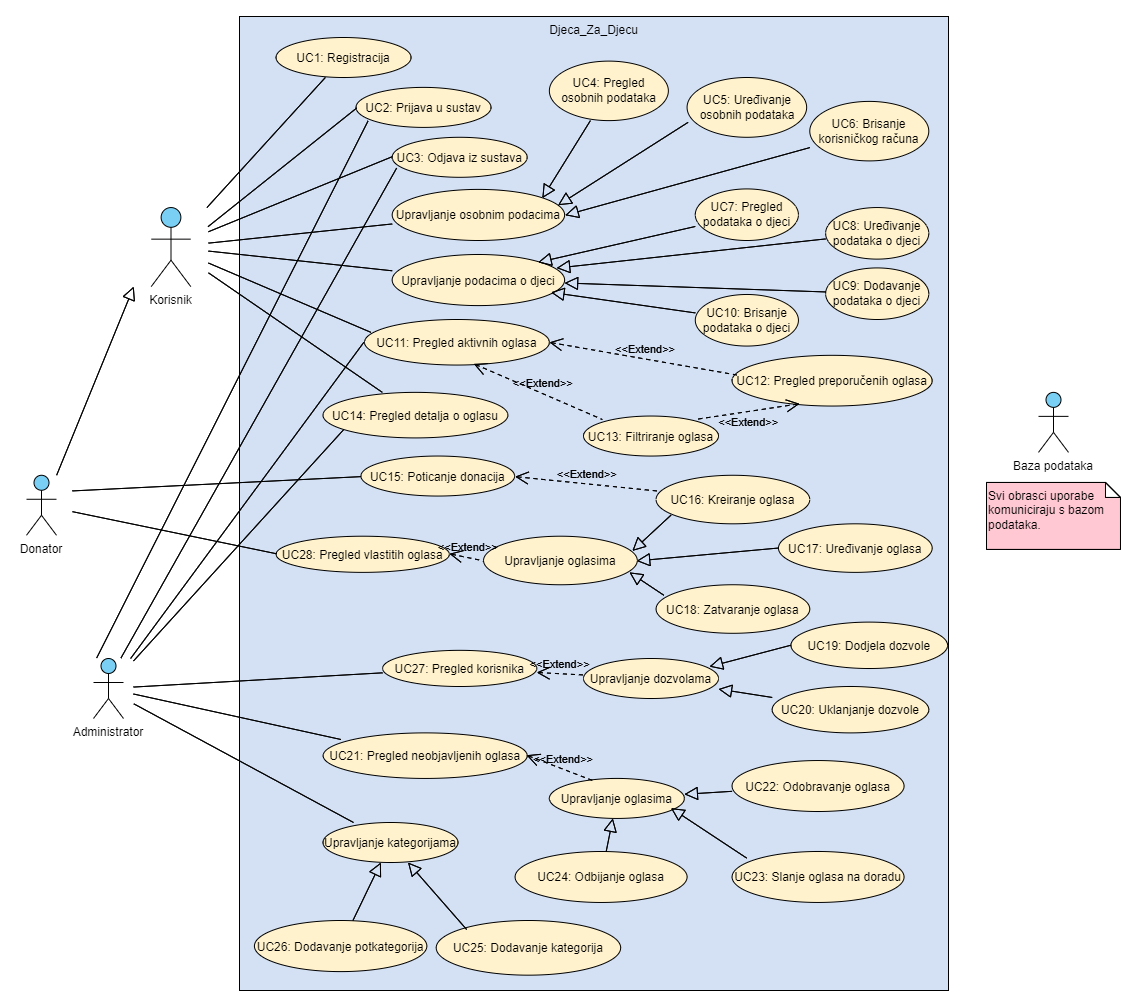
\includegraphics[width=\textwidth,height=0.7\textheight]{dijagrami/UCD - Djeca za djecu.png}
						\centering
						\caption{Dijagram obrazaca uporabe - aplikacija Djeca za djecu}
						\label{fig:useCaseDiagramMain}
					\end{figure}
					%\textit{Prikazati odnos aktora i obrazaca uporabe odgovarajućim UML dijagramom. Nije nužno nacrtati sve na jednom dijagramu. Modelirati po razinama apstrakcije i skupovima srodnih funkcionalnosti.}
				\eject
				
			\subsection{Sekvencijski dijagrami}
				\begin{figure}[H]
						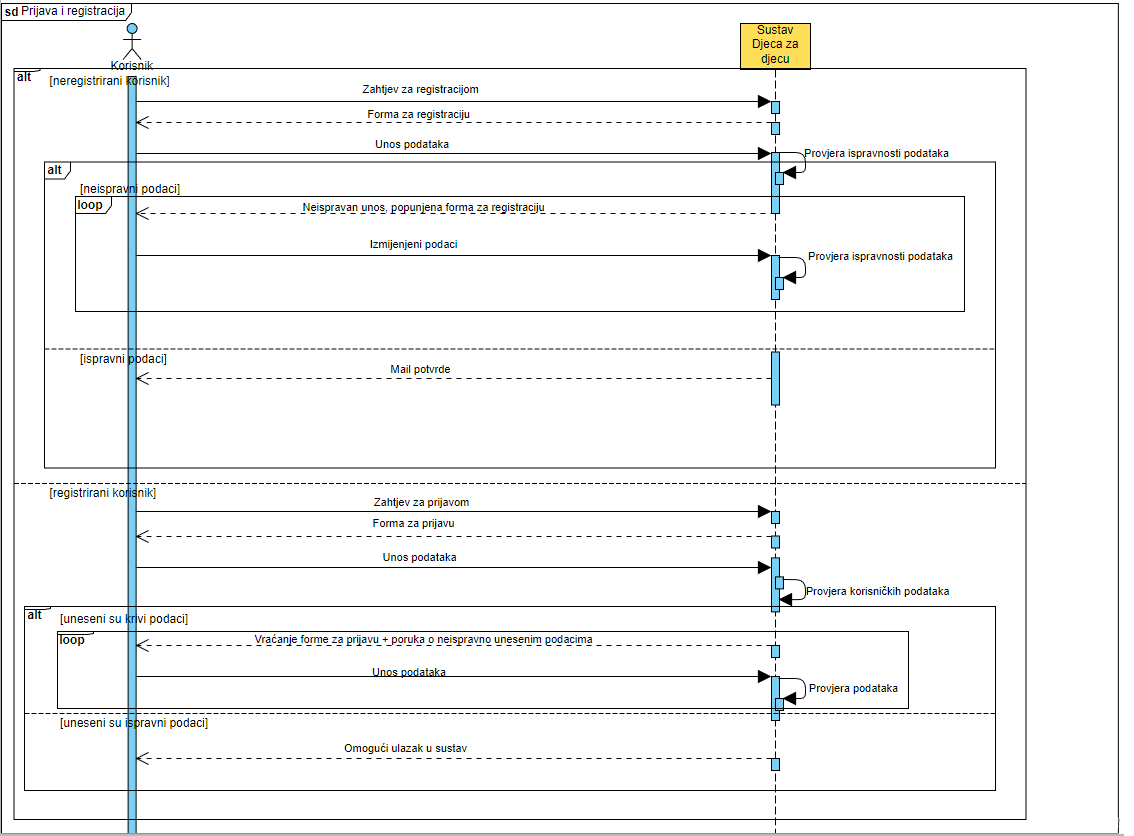
\includegraphics[width=\textwidth,height=0.7\textheight]{dijagrami/sq_d_pr_reg.png}
						\centering
						\caption{Sekvencijski dijagram - prijava i registracija}
						\label{fig:Prijava i regirtracija}
				\end{figure}
				\textit{Dijagram prikazuje početni zaslon tj. opcije početnog zaslona kada korisnik pristupi aplikaciji. Korisnik ima dvije opcije, ako je neregistriran mora otići na registraciju (klikom miša) i tada mu se prikazuje forma za registraciju koju treba popuniti i poslati sustavu klikom na gumb potvrde. Sustav provjerava ispravnost unesenih podataka slanjem u bazu podataka koja sustavu šalje odgovor o ipsravnosti. Postoji mogućnost da su uneseni podaci neispravni. U tom slučaju sustav vraća formu korisniku na popravljanje i korisnik izmjenjene podatke treba ponovo poslati sustavu koji će ih provjeriti (na isti način već opisan gore). Taj slučaj se može ponoviti onoliko puta dok uneseni podaci nisu ispravni. Ispravno uneseni podaci znače da sustav šalje mail potvrde, sada, registriranom korisniku.\\ Registrirani korisnik može klikom na gumb za prijavu poslati sustavu zahtjev za formu za prijavu koju treba ispuniti kad mu se prikaže(sustav je pošalje). Uneseni podaci se provjeravaju u bazi korisnika u sustavu. Ako su ovdje uneseni podaci krivi korisniku se šalje forma za prijavu kao i poruka o neispravno unesenim podacima. Dok podaci nisu ispravni ovaj korak se ponavlja. Kada su podaci ispravno uneseni sustav omogućava ulazak u sustav(preusmjerava na stranicu s oglasima)}
				\newline
				
				\begin{figure}[H]
						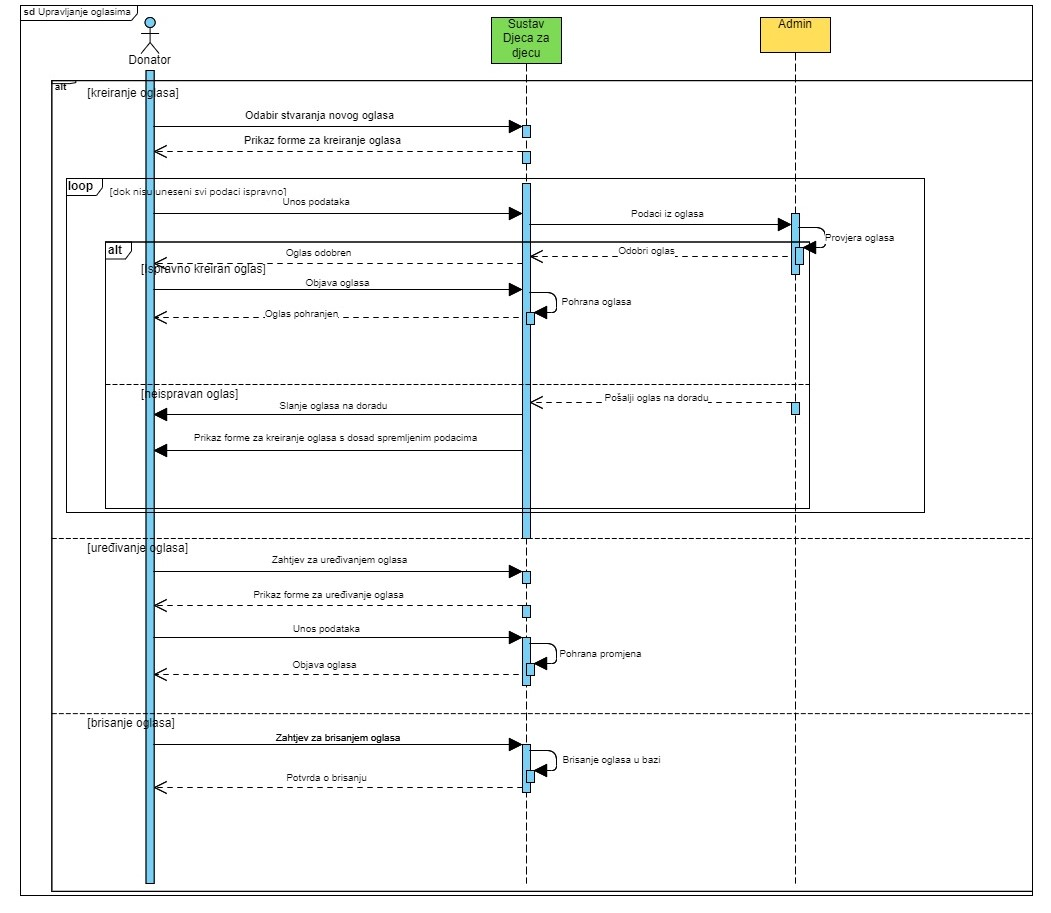
\includegraphics[width=\textwidth,height=0.7\textheight]{dijagrami/sqd_upr_ogl.png}
						\centering
						\caption{Sekvencijski dijagram - upravljanje oglasima}
						\label{fig:Upravljanje oglasima}
				\end{figure}
				\textit{Dijagram prikazuje upravljanje oglasima koje je omogućeno donatorima (korisnici koji su od Administratora dobili dozvolu za doniranjem). Donator ima tri opcije koje može odabrati. Ukoliko odabere opciju kreiranja oglasa sustav mu šalje formu za kreiranje oglasa. Korisnik unosi podatke o predmetu koji oglašava toliko dugo dok nisu potvrđeni. Unešene podatke sustav šalje Adminu na provjeru koji potom sustavu javlja treba li ih poslati korisniku na doradu, javiti korisniku da je oglas odobren ili čak odbiti. U slučaju dorade donatoru sustav šalje njegovu formu s podacima o oglasu i gornji koraci se provode ponovo. Ako je oglas odobren donator može objaviti oglas u sustavu koji taj oglas pohranjuje i šalje potvrdu donatoru o objavi oglasa. Kad je oglas odbijen on se odbacuje i korisnik dobiva obavijest o odbijanju oglasa. \\Kod uređivanja oglasa korisnik sustavu šalje zahtjev za uređivanjem određenog oglasa i sustav odgovara slanjem forme za uređivanje oglasa. Donator unosi podatke i oni se pohranjuju u sustav te se ponovno objavljuje oglas. \\Opcija zatvaranja oglasa podrazumijeva slanje zahtjeva za zatvaranjem oglasa. Po primitku zahtjeva sustav zatvara oglas i vraća korisniku potvrdu o zatvorenom oglasu. }

				\eject				

			
				%\textbf{\textit{dio 1. revizije}}\\
				
	
		\section{Ostali zahtjevi}
			\begin{packed_item}
				\item Sustav treba podržavati istovremenu aktivnost više korisnika
				\item Aplikacija treba biti responzivna tj. prilagođena uređajima svih rezolucija (tableti, mobiteli) 
				\item Aplikacija treba biti jednostavna za korištenje i imati intuitivno sučelje
				\item Aplikacija treba biti implementirana u arhitekturi klijent-poslužitelj
				\item Poslužiteljska strana aplikacije mora biti implementirana koristeći jezik Javu i radni okvir Spring Boot
				\item Podaci trebaju biti spremani u bazu podataka koristeći Java Persistance API (JPA)
				\item Funkcionalnosti poslužiteljske strane aplikacije trebaju biti izložene kroz REST Web servise
				\item Klijentska strana aplikacije mora biti implementirana koristeći tehnologije Angular ili React
			\end{packed_item}
		 